\section{Introduction}

The goal of information extraction (IE) \cite{Grishman1997} is to extract
structured information
from unstructured or semi-structured data. Relation extraction (RE) \cite{Bach} is an 
important branch of IE, which aims at extracting
relations (usually binary) between entities from a natural language
sentence. When the target
relation is binary, the result of RE is in the form of ($e_1$, $r$, $e_2$) 
triples. One of the most important use of such relation triples
is to construct knowledge graphs, which forms the basis 
of many downstream NLP tasks such as question answering (QA) \cite{Bao2014}, 
and information retrieval (IR) \cite{Castells2007}.



RE is a challenging task and still far from being solved due to the 
variety and ambiguity of natural language. \YY{Find a reference}
\figref{fig:triple-eg} illustrates the RE task. The target sentence contains 4 named 
entities, i.e., ``Tim Cook'', ``Apple'', ``Beijing'', and ``China'', and
2 types of relations, namely ``LeaderOf'' and ``CityOf''. One of the relation
triples is \{Tim Cook, LeaderOf, Apple\},  where $e_1$ is a person entity 
``Tim Cook'', $r$ is ``LeaderOf'', and $e_2$ is ``Apple''. We also call
$e_1$ and $e_2$ an \emph{entity pair} for a relation triple. 
The \emph{relation type} $r$ is used to indicate the semantic relationship
between the two entities in \emph{entity pair}. 
In other word, a relation triple
contain two kind of information: entity information carried by
\emph{entity pair}, and relationship information carried by
\emph{relation type}.



\begin{figure}[th]
\centering
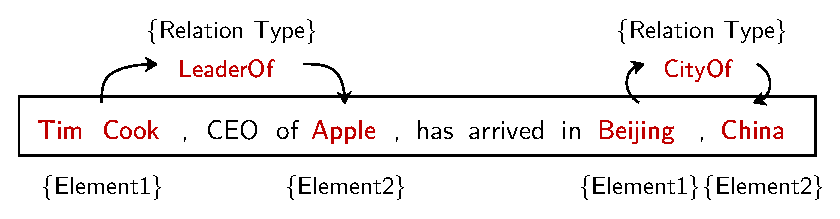
\includegraphics[width=\columnwidth]{pictures/introduction.eps}
\caption{A Gold standard example. This sentence contains 2 relation triple, \{
  Tim Cook, LeadOf, Apple\} and \{ Beijing, CityOf, China\}.
  \label{fig:triple-eg}}
\end{figure}



Traditionally, the problem of RE has been treated as a sequence of two
sub-tasks, namely named entity recognition (NER) \cite{Nadeau2007} and relation
classification (RC) \cite{Zeng2014}.
Solving RE amounts to first recognizing the
named entities in the sentence, and then determining the relation type
between these entities. The latter sub-task of RE depends on the result of
NER. In the past, the most successful approaches to solve RE come from
machine learning and they fall into two categories, pipelined
\cite{Zeng2014,Wang2016,Wen2017,Cai2016,Zhou2016,Xu2015}
and joint approaches
\cite{Zheng2017a,Li2017a,Li2014,Adel2017,Gupta2016,Miwa2014,Kate2010,
  Miwa2016,Katiyar2017,Ren2017}. Pipelined approaches treat NER and RC as two
separate tasks and trains two independent models. The obvious
drawback of this approach is that the training of NER or RC cannot benefit
each other, when in reality the two sub-tasks are inter-dependent \YY{Need a
  reference}. This inspires the second category of approaches which train the
two models jointly by sharing some common, low-level parameters. 
This type of joint-learning
showed some advantage against the first approach and gained popularity lately.
However, the joint approaches still produce two models and they
are used sequentially at prediction time. Such a two-step RE approach has
two disadvantages. First, error can propagate from NER to RC. 
For example, if ``Apple'' is incorrectly recognized as a ``Location'' entity 
in the NER part, it is impossible for the RC part to classify entity pair 
(Tim Cook, Apple) to ``LeaderOf'' relation. Second, although joint approaches
share the low-level parameters between NER and RC, these two sub-tasks can not
make full use of high level feature from each other. For example, if the RC part
knows that the pattern ``CEO of'' implies with
high probability the relation type ``LeaderOf'', then there's a high chance that
``Tim Cook'' is a person while ``Apple'' is an organization.



To address the above challenges of a two-step approach, 
\citet{Zheng2017}
proposed to view RE as a normal sequence tagging problem and
thus do away with the two sequential sub-tasks. 
This new approach infers for each word in a
sentence a special tag that contains both entity and relation information. 
Once the words in a sentence is tagged, we can then reconstruct
relation triples without the NER and RC steps at all.
While this idea is great, the popular model for sequence tagging, namely,
recurrent neural networks, which Zheng et al. used in their work, has its
own limitations. First, it cannot make use of the entities that do not take
part in the relation triples in the sentence since these are simply labeled
as ``others'' in the training data. Second, RNN and its variants make tagging
prediction largely based on local or contextual information and ignores 
global information that might be helpful in the sentence.


%  \textbf{Here, we call
% the model of \cite{Zheng2017} basic RE tagging model, and ours joint RE tagging model.}

To this end, in this paper, we proposed to augment the model 
of \citet{Zheng2017} with an new task to reinforce that model by joint learning. 
%The first task is simply NER which is helpful to catch complete entity 
%related features to the sequence labeling problem. 
The new task is called relation type detection 
(RTD) which extracts relation type features for the RE tagging problem.
RTD differs from RC is that RC predicts one relation type given a pair of entities,
while RTD detects all possible relation type in a sentence without the knowledge
of entities. Because a sentence may contain multiple relations, RTD is a multi-label
classification problem.
In our setting, RE tagging is the main task while RTD is an {\em auxiliary
task} which assists the main task by providing useful features.


The main contributions of our work is as follows.
\begin{itemize}
\item We propose a novel multi-task learning model that treats RE as a global
sequence tagging problem but reinforce it with an auxiliary task (\secref{sec:tagging},
\secref{sec:train}).
\item We propose a more effective algorithm to re-construct triples from relation
  tag sequence (\secref{sec:triple}).
\item Our results show that the new model achieves up to 14\% gain on end-to-end 
RE accuracy over the state-of-the-art models (\secref{sec:eval}). 
\end{itemize}

